\documentclass[10pt,twocolumn,letterpaper]{article}

\usepackage{cvpr}
\usepackage{times}
\usepackage{epsfig}
\usepackage{graphicx}
\usepackage{amsmath}
\usepackage{amssymb}
\usepackage{adjustbox}
\usepackage[center]{caption}

\usepackage[backend=bibtex,style=verbose-trad2]{biblatex}

% Include other packages here, before hyperref.

% If you comment hyperref and then uncomment it, you should delete
% egpaper.aux before re-running latex.  (Or just hit 'q' on the first latex
% run, let it finish, and you should be clear).
\usepackage[breaklinks=true,bookmarks=false]{hyperref}

\cvprfinalcopy % *** Uncomment this line for the final slatexubmission

\def\cvprPaperID{****} % *** Enter the CVPR Paper ID here
\def\httilde{\mbox{\tt\raisebox{-.5ex}{\symbol{126}}}}

% Pages are numbered in submission mode, and unnumbered in camera-ready
%\ifcvprfinal\pagestyle{empty}\fi
\setcounter{page}{1}
\begin{document}

%%%%%%%%% TITLE
\title{Applying RBF Support-Vector Regression to Forecast the Inflation Rate with Disaggregated Sector Data  }

\author{Jungang Li\\
Economics Department\\
University of Oregon\\
{\tt\small jungangl@uoregon.edu}
% For a paper whose authors are all at the same institution,
% omit the following lines up until the closing ``}''.
% Additional authors and addresses can be added with ``\and'',
% just like the second author.
% To save space, use either the email address or home page, not both
%\and
%Second Author\\
%Institution2\\
%First line of institution2 address\\
%{\tt\small secondauthor@i2.org}
}

\maketitle
%\thispagestyle{empty}

%%%%%%%%% ABSTRACT
\begin{abstract}
The inflation rate is monitored closely by the central banks as an important macroeconomic factor for major policy changes. Increasing the accuracy of the inflation rate gives policymakers a better outlook of the economy. The headline inflation rate is calculated based on a fixed basket of goods, and these goods can further be categorized into different sectors. Time series leave-one-out cross-validation is used to tune the hyper-parameters of each model.  
\end{abstract}
%%%%%%%%% BODY TEXT
\section{Introduction}
Inflation is one of the few critical economic variables for monetary policymakers. There is a vast literature on forecasting aggregate inflation, given the importance of these forecasts for monetary policy. There are a large number of variables that may be helpful for forecasting inflation. Putting all these variables into the model leads to low accuracy of out of sample forecasts. There are two problems when we add too many RHS variables into a model: (1) overfitting in the sample, and (2) low degrees of freedom. Recent studies have shown that dynamic factor models may provide a parsimonious way to include incoming information about a wide variety of economic activity such as Stock and Watson (1999, 2002), Bernanke and Boivin (2003), Bernanke, Boivin, and Eliasz (2005) and Giannone, Reichlin, and Sala (2005). 

\section{Data and the General Model}
\begin{figure*}[t]
\begin{center}
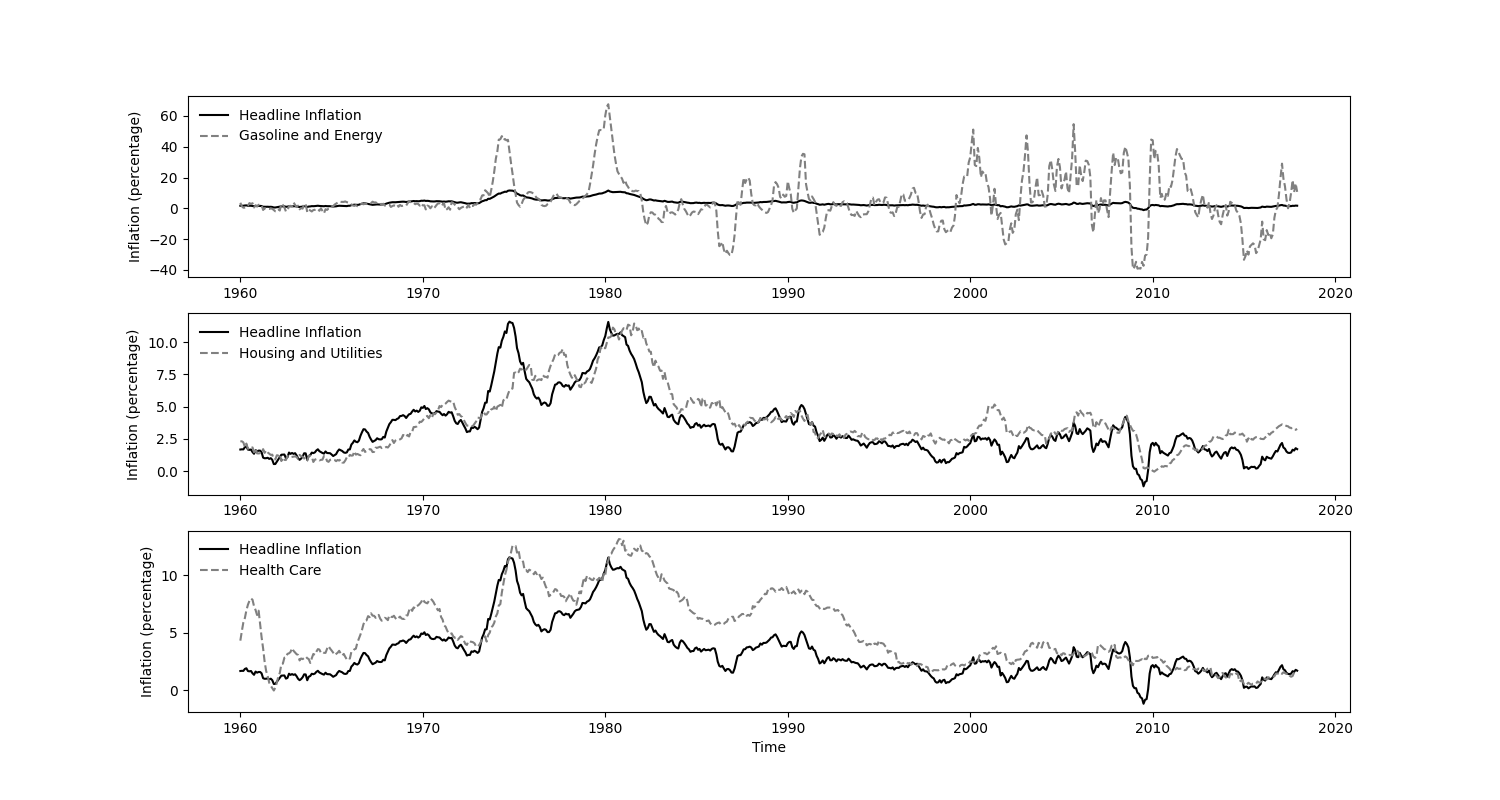
\includegraphics[scale=0.5]{../../Python/Times_Series.png}
\caption{The Headline Inflation Rate v.s. Disaggregated Inflation Rates}
\end{center}
\end{figure*}

This paper explores the potential use of recently developed techniques in the machine learning literature and compares the performance of various models (including dynamic factor models.) This paper contributes to the literature by evaluating different novel forecast modeling strategies from machine learning literature. Some literature investigates using disaggregated information on inflation to forecast the aggregate inflation rate. A few papers also have explored the implementation of machine learnings to predict the inflation rate. Still, this project is the first to combine the disaggregated data with deep learning algorithms.

The U.S. Bureau of Economic Analysis collects both the headline consumer price index and the indexes by sectors. For example, the personal consumption expenditure (PCE) can be divided into fifteen different segments: vehicles, furnishings and durables, recreational goods, other durables, groceries, clothing and footwear, gasoline and energy, other nondurables, housing and utilities, health care, transportation services, recreational services, food services and accommodations, financial services, other services, donations. The intuition of leveraging disaggregated data is that it takes time for the inflation of prices in one sector to impact the headline aggregate inflation rate fully. For the nature of supply chain contracts, the transportation companies usually purchase gas from the oil companies at a negotiated rate that is fixed for a certain amount of time. The increase in oil prices will eventually spread into the other sectors over time. Hence, the inflation of gasoline and energy could be used to forecast the future headline inflation rate. 

I consider one baseline model and three machine learning models. The baseline model is a simple autoregressive model of order 1, \textit{a.k.a} AR(1) model. The three machine learning models are support vector regression model (SVR), Lasso Regression, and Ridge Regression (RR). I tend to find the answers to the following questions. Which kernel should be used for the Support Vector Regression?  Which sectors have the prediction power according to the Lasso and Ridge Regression? Which machine learning model has the best performance? Will machine learning models improve the forecasting accuracies compared to the baseline model?

The rest of the paper is organized as follows: Section 2 describes the data and the general forecasting model; Section 3 provides the details of the regression models with their regularization parameters and the accuracy function; Section 4 covers the experiments with time series cross-validations for tuning the hyperparameters for each model and shows the results; Section 5 gives conclusions. 



The Personal Consumption Expenditure Price Index (PCEPI) is aggregated from price indexes of a large number of underlying goods and service categories. PCEPI is a United States-wide indicator of the average increase in prices for all domestic personal consumption. It is bench-marked to a base of the year 2009 = 100. I have downloaded the aggregated and disaggregated data from the Federal Reserve Bank of St. Louis. Let the $P_{i, t}$ be the CPI for $i$ at month $t$ where $i$ denote either the aggregate personal consumption or a sub-category, the inflation rate for $i$ at month $t$ can be computed as $\Pi_{i, t} = 100(P_{i, t} - P_{i, t-12})/P_{i, t-12})$. The CPI data runs monthly from 1959 Jan to 2017 Dec. The inflation data runs from 1960 Jan to 2017 Dec because the first 12 months are used to calculate the rate of change. I select three disaggregated inflation rates to compare with the inflation rate for personal consumption (headline inflation). The comparisons are shown in Figure 1. We can see that the movement of gasoline and energy inflation precedes the headline inflation, housing, and energy inflation movements follow the headline inflation. In contrast, healthcare inflation moves with the headline inflation rate mostly concurrently. 

Following the conventions of the forecasting literature, set the model to forecast the average inflation rate for twelve months ahead. For example, standing in December 2017, the forecasting problem is to forecast the average inflation rate for the period between January 2018 to December 2018. The general formation of the models to be considered is $\hat \Pi_{a, t+12} = \hat f(X_{t})$ where $X_{t}$ is the features used in the forecasting model at time $t$. For the baseline model, $X_{t}$ only includes $\Pi_{a, t}$ which \noindent is the aggregate inflation rate. For the machine learning models, $X_{t}$ includes both  $\Pi_{a, t}$ and $\{\Pi_{i ,t}\}_{i = 1}^{15}$ which are the $15$ disaggregated inflation rates. 
Another salient characteristic of the inflation data is that it shows two distinct eras: the great inflation and great moderation. In economics, the great moderation is the reduction in the volatility of business cycle fluctuations in the United States starting in the mid-1980s. Former Federal Reserve chair Volcker implemented a series of contractionary monetary policies to reduce the high inflation rates during the 70s. Another significant change in the inflation process is the 2008 great recession, where the inflation dropped quickly and bounced back. 

\begin{figure*}[t]
\begin{center}
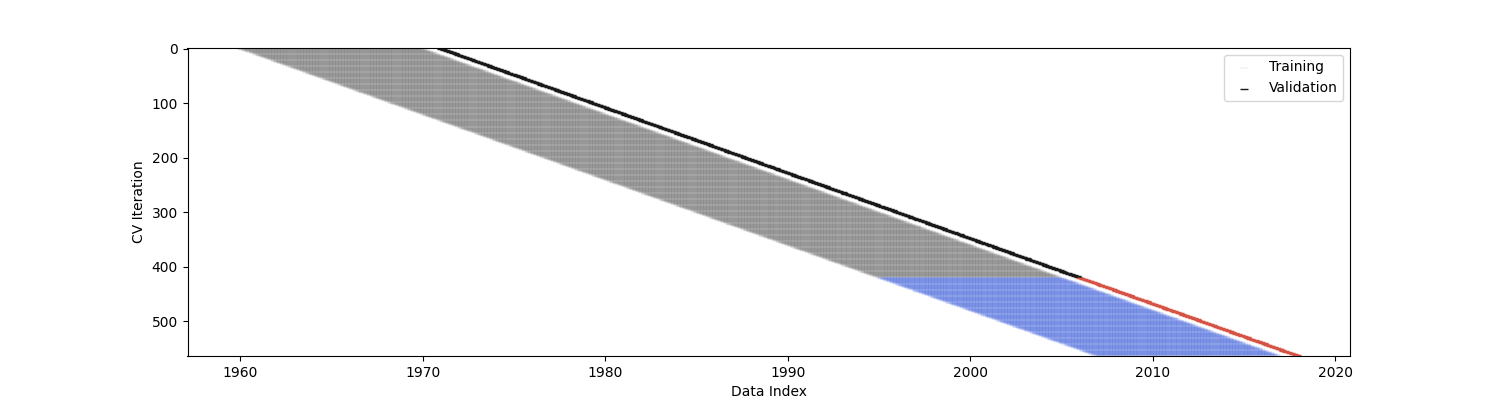
\includegraphics[scale=0.5]{../../Python/TimeSeriesSplit.png}
\caption{Time Series Leave -One-Out Cross-Validation Data Splits}
\end{center}
\end{figure*}

\section{Regression Models and RMSE}
For the baseline autoregressive model, only the lagged headline inflation is used as the regressor. For the machine learning regression models, I include all fifteen disaggregated inflation rates as the regressors besides the headline inflation rate. I use the canned functions in the \textit{sklearn} python package to set up the regression models. The regression accuracy is evaluated using the negative of the root mean squared error which takes the form of $RMSE = \sqrt[2]{||\hat y - y||^2}$ where $\hat y$ is the model-predicted inflation rate from the testing data set and $y$ is the corresponding ground-truth inflation rate. There is no hyper-parameter to tune for the simple autoregressive model. The hyperparameter for the support vector regression model is the coefficient $C \geq 0$ for the soft margin. Notably, there is another hyperparameter $ \gamma $ that controls the sharpness of the boundary for radial basis function kernel in the SVR. Instead of minimizing the observed training error, SVR reduces the generalization error bound. The hyperparameters for lasso and ridge regression models are the coefficients $\alpha \geq 0$ for L1 and L2 regularization terms. Ridge and Lasso shrink the coefficients to reduce the model complexity and multi-colinearity. These hyperparameters control over-fitting of the regression models, which will be tuned over the validation data set.

Furthermore, for the support vector regression model, I consider four different kernels: linear, quadratic, radial basis function, and sigmoid. To tune to hyperparameters, I used time series hold-one cross-validation, illustrated in Figure 2. Shuffling in cross-validation is not appropriate because we want to preserve the serial relations between the data. This is a variation of K-fold cross-validation in the sense that we always use the first K folds as the training set and the K+1 fold as the test set. Successive training sets are supersets of those that come before them. 
To evaluate the performance of the tuned models, I hold out the data from January 2005 to December 2017 as the test set. The hold-out ground truth inflation rates are colored red in Figure 2, while the blue color indicates the data used to train the tuned regression model. When the model trains, it only uses the previous ten years of data or 120 data points. This choice is made to avoid the biases introduced by the structural change across time. 

\section{Experiments}
Each regression model is tuned according to the development data set that runs from January 1950 to December 2004 (660 data points). I split the whole 660 data points 408 times. The first split uses the lagged inflation rates of the index from January 1960 to December 1970 to forecast the 12-month ahead headline inflation rate indexed in January 1971, representing the average inflation rate in 1970. The last split in the development date uses the lagged inflation rates of the index from December 1993 to November 2003 to forecast the 12-month ahead headline inflation rate indexed in December 2004, which represents the average inflation rate during 1970. For the hold-out data set, I predict the inflation rate from January 2005 to December 2017.

The finding is that support vector regression model with radial basis function kernel outperforms the other regression models by a large margin. From preliminary experiments, root mean squared errors for each of the models can be summarized as follows
\begin{center}
\footnotesize
\begin{tabular}{ |c|c|c|c| } 
 \hline
 Model & Hyperparameter & Dev RMSE & Hold-out RMSE \\ 
 \hline
 AR(1) & N/A & $2.7715$ & $1.2626$\\ 
Ridge & $\alpha = 0$ & $0.8429$ & $0.7663$ \\ 
Lasso & $\alpha = 0$ & $0.8742$ & $0.7658$ \\
SVR(RBF) & $C = 77, \gamma = 0.0035$& $0.2594$& $0.4439$\\
\hline
\end{tabular}
\end{center}

\begin{figure*}[t]
\begin{center}
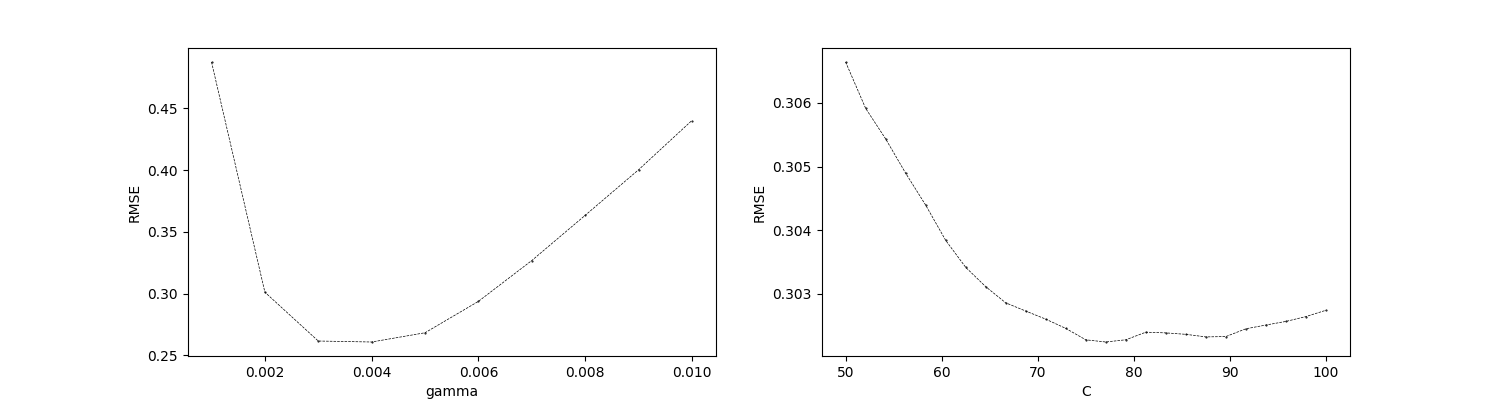
\includegraphics[scale=0.5]{../../Python/Tuning_SVR.png}
\caption{Tuning the hyperparameters for SVR}
\end{center}
\end{figure*}

The autoregressive model performs poorly compared to Ridge and Lasso, which utilize the information in the disaggregated data. This shows that the disaggregated inflation rates have the power to increase forecasting accuracy, and the Ridge and Lasso models can utilize this information. Focus on the novel finding of this project, namely increasing the inflation forecast accuracy via the SVR model with RBF kernel. This model has two hyperparameters to tune. For illustration purposes, I use a greedy algorithm to tune these two parameters. The procedure is first to find $C$ that minimizes RMSE, fixing $\gamma$ at the default level, which is $\frac{1}{N \cdot X_{var}()}$ where $N$ is the feature number which is $16$ in this case. After that, I find the $\gamma$ that minimizes RMSE, fixing $C$ at the optimal level. I only repeat the process only once to avoid overfitting the model. The tuning process result can be shown in Figure 3. One remarkable result is that the SVR model performs extremely well compared to the other models. For the training set, SVR yields a very low RMSE that is as low as $0.26$, which is four times better than the second-best regression model (Ridge). For the hold-out period, SVR still dominates the second-best with an RMSE as low as $0.444$, which is $75\%$ more accurate than the ridge regression model for the same hold-out data. To illustrate the huge difference in terms of forecasting performance between SVR and Ridge, I plot the inflation forecast side by side with the true inflation rate in Figure 4 and Figure 5. I make a few comments about the behaviors of the SVR regression:

\begin{enumerate}
\itemsep0em 
\item Considering the long forecast horizon (12 months), SVR performs wells in terms of forecast accuracy. 
\item For the hold-out data, SVR performs better during low inflation periods. That is the period excluding the 2008 great recession. 
\item The SVR model performs very well during the great inflation period in the 70s.
\item A few ``over-shooting" behaviors are observed for SVR when the inflation rate is coming back up. 
\end{enumerate}

\section{Conclusion}
Support vector regression use kernels to handle nonlinearity in the data and use a maximum margin algorithm. I find that the best kernel for forecasting inflation rate is the radial basis function kernel, which outperforms the other kernels and other regression models by a large margin ($75\%$ better than the second-best in the hold-out data). For future research, it would be interesting to see which disaggregated inflation rate has the most significant prediction power in improving the forecast accuracy. Another research direction would be investigating the level of disaggregation. This paper only considers a relatively shallow level where personal consumption is divided into $15$ categories. Future research can investigate whether a deeper disaggregation level could further improve forecasting accuracy. Finally, the mechanism of why SVR models have excellent performance is also worth studying.

In conclusion, I show that the central banks and other financial institutions can use machine learning models, especially support-vector regression models, to improve their accuracy of inflation forecast. For robustness, data sets from Europe and Japan can also be used under SVR models to check this finding's universality. Other fields where disaggregated data are available such as forecasting the S\&P 500 index using industry indexes in the stock market, can also be a promising field for applying SVR. 

\begin{figure*}
\begin{center}
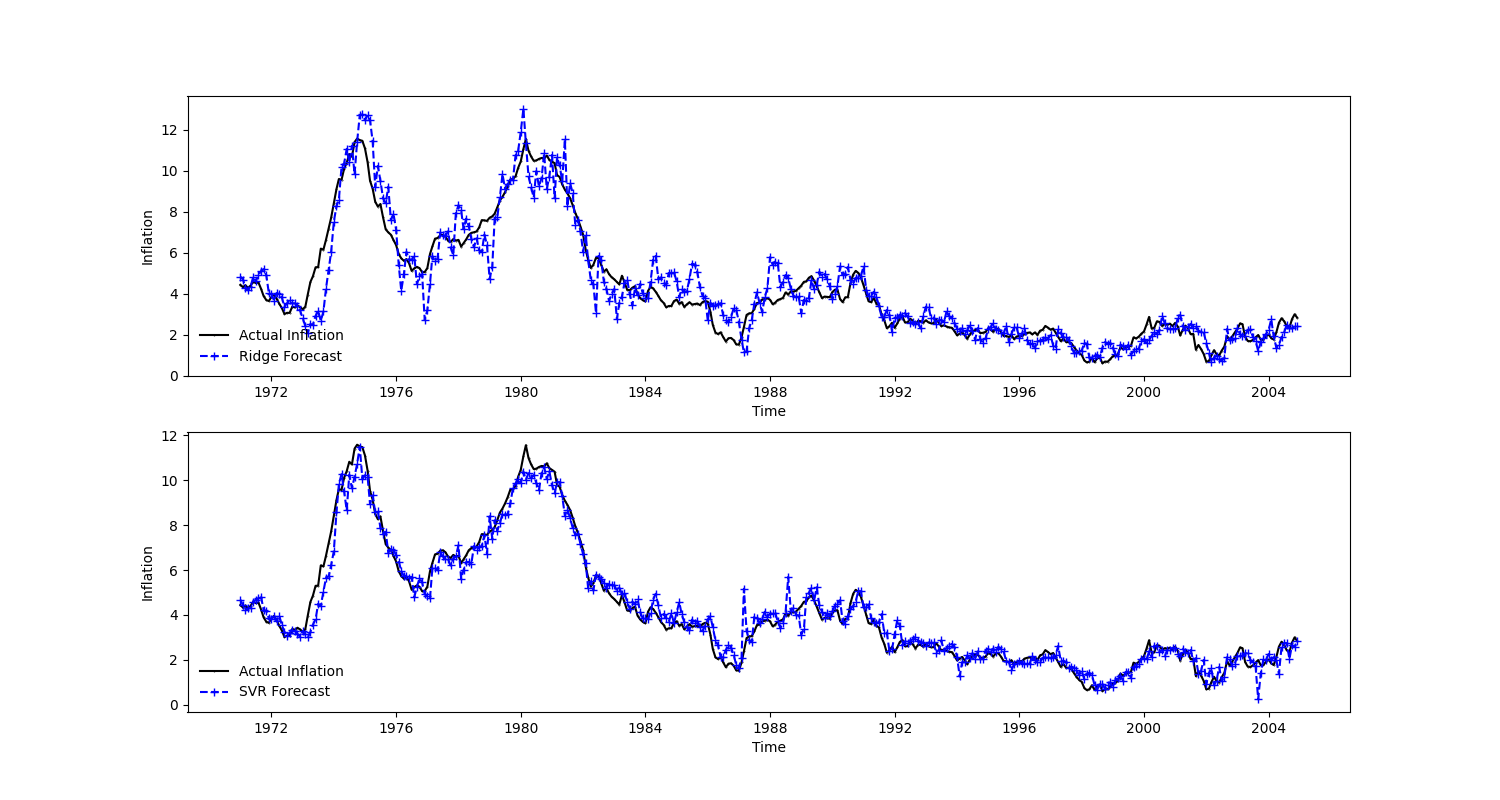
\includegraphics[scale=0.48]{../../Python/Forecast_Dev.png}
\caption{Inflation Forecast in Development Data}
\end{center}
\end{figure*}

\begin{figure*}
\begin{center}
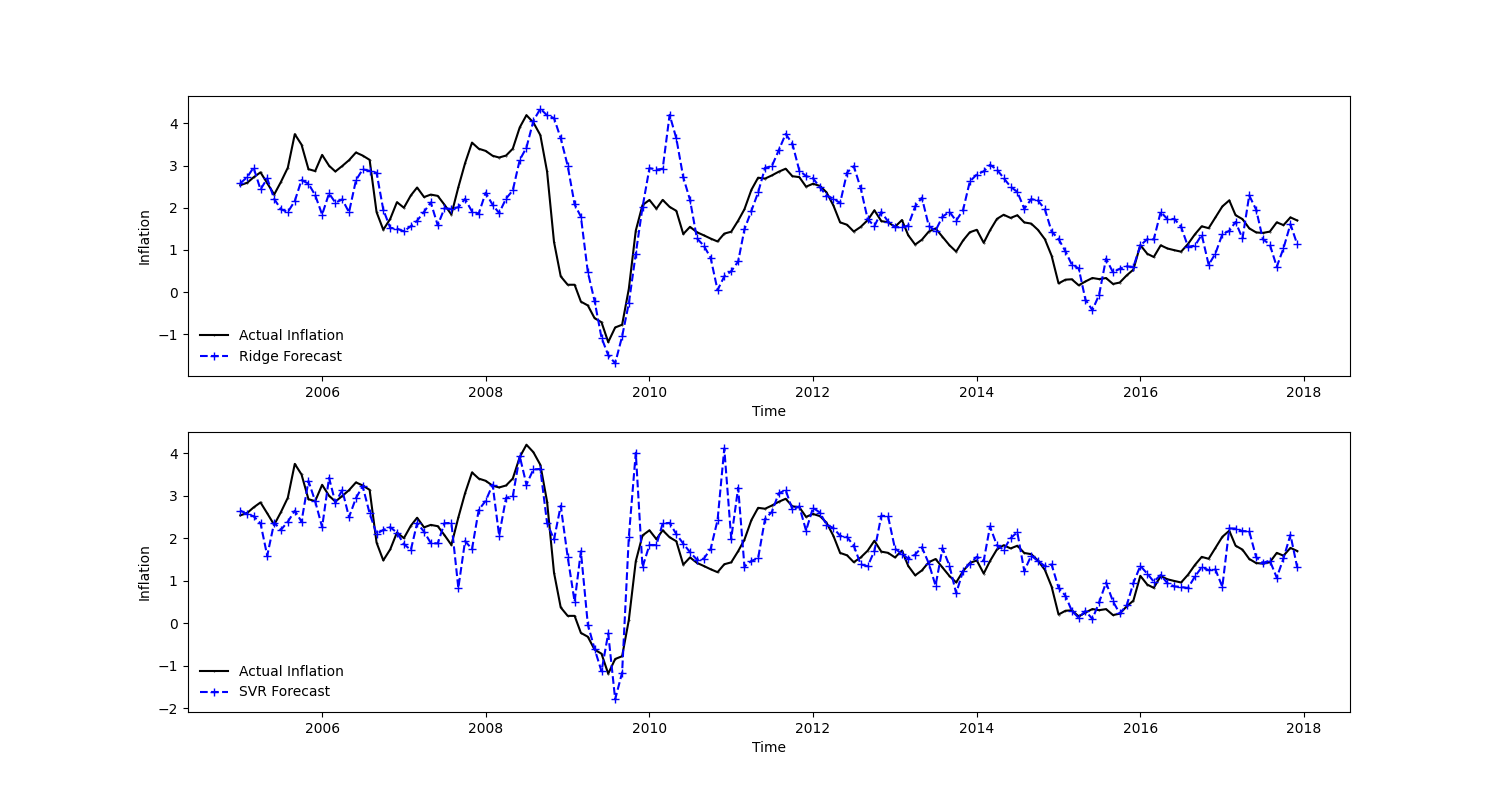
\includegraphics[scale=0.48]{../../Python/Forecast_HO.png}
\caption{Inflation Forecast in Hold-out Data}
\end{center}
\end{figure*}



\begin{thebibliography}{9}
\bibitem{latexcompanion} 
Ahmed, Nesreen K, Atiya, Amir F, Gayar, Neamat El, and El-Shishiny, Hisham.
\textit{An empirical comparison of machine learning models for time series forecasting}. 
 Econometric Reviews, 29(5-6), 594–621, 2010. 

\bibitem{latexcompanion} 
Alvarez, Marcos, and Gupta, Rangan.
\textit{Forecasting US consumer price index: does nonlinearity matter?}
Applied Economics, 48(46), 594–621, 2016. 

\bibitem{latexcompanion} 
Stock, J. H., and Watson, M. W.
\textit{Forecasting Inflation}. 
Journal of Monetary Economics, 44, 293-335., 1999. 
 
 \bibitem{latexcompanion} 
Stock, J. H., and Watson, M. W.
\textit{Macroeconomic Forecasting Using Diffusion Indexes}. 
Journal of Business and Economic Statistics, 20, 147-162., 2002. 
 
\end{thebibliography}

\end{document}

